\chapter{Algebraic curves in the projective plane}
\section{Homogenisation of plane curves}
Take a plane algebraic curve \(y^2=x^2+x^3\) in the affine plane over a field \(k\).
\begin{center}
\documentclass{standalone}
\usepackage{tikz}
\usepackage{pgfplots}
\usepackage{xparse}
\pgfplotsset{compat=1.14}%
\colorlet{curveZero}{gray!85}
\colorlet{curveOne}{blue!60}
\definecolor{curveOneColor}{rgb}{.6,0,0}
\colorlet{curveTwo}{brown!50!gray}
\colorlet{curveThree}{green!40!gray}
\colorlet{curveFour}{red!50!gray}
\NewDocumentCommand\DrawDotInPlot{O{}mmO{}}%
{%
\fill[gray!15,draw=gray] (axis cs:{#2},{#3}) circle [radius=1.6pt] node[above,black,#4] {\(#1\)};%
}%
\NewDocumentCommand\DrawDot{O{}mmO{}}%
{%
\fill[gray!20,draw=gray] ({#2},{#3}) circle (1.6pt) node[above,black,#4] {\(#1\)};%
}%
\NewDocumentCommand\DrawNode{O{}m}%
{%
\fill[gray!20,draw=gray] (#2) circle (1.6pt) node[above,black] {\(#1\)};%
}%
\NewDocumentCommand\DrawDotThreeD{O{}mmmO{}}%
{%
\fill[gray!20,draw=gray] ({#2},{#3},{#4}) circle (1.6pt) node[above,black,#5] {\(#1\)};%
}%
\colorlet{axisColor}{gray!50}
\tikzstyle{shapeZero}=[fill=curveZero,opacity=.4]
\tikzstyle{shapeOne}=[fill=curveOne,opacity=.4]
\tikzstyle{shapeTwo}=[fill=curveTwo,opacity=.4]
\tikzstyle{shapeThree}=[fill=curveThree,opacity=.4]
\tikzstyle{groupElementLabel}=[minimum size=2.4em]
\tikzstyle{groupElement}=[minimum size=2.4em,shapeZero,draw=curveZero]
\tikzstyle{cosetOne}=[minimum size=2.4em,shapeOne,draw=curveOne]
\tikzstyle{cosetTwo}=[minimum size=2.4em,shapeTwo,draw=curveTwo]


\begin{document}

\begin{tikzpicture}
\begin{axis}[hide axis,xmin=-2,xmax=2,ymin=-2,ymax=2,width=4cm]
  \addplot[very thick,domain=-1:0,curveZero,samples=200]{sqrt(x^2+x^3)};%
  \addplot[very thick,domain=-1:0,curveZero,samples=200]{-sqrt(x^2+x^3)};%
  \addplot[very thick,domain=0:1,curveZero]{sqrt(x^2+x^3)};%
  \addplot[very thick,domain=0:1,curveZero]{-sqrt(x^2+x^3)};%
\end{axis}
\end{tikzpicture}
\end{document}

\end{center}
The \emph{cone}\define{cone} on the curve is the surface in \(k^3\) whose points \((x,y,z)\) satisfy the homogenization \(y^2z = x^2z + x^3\).
\begin{center}
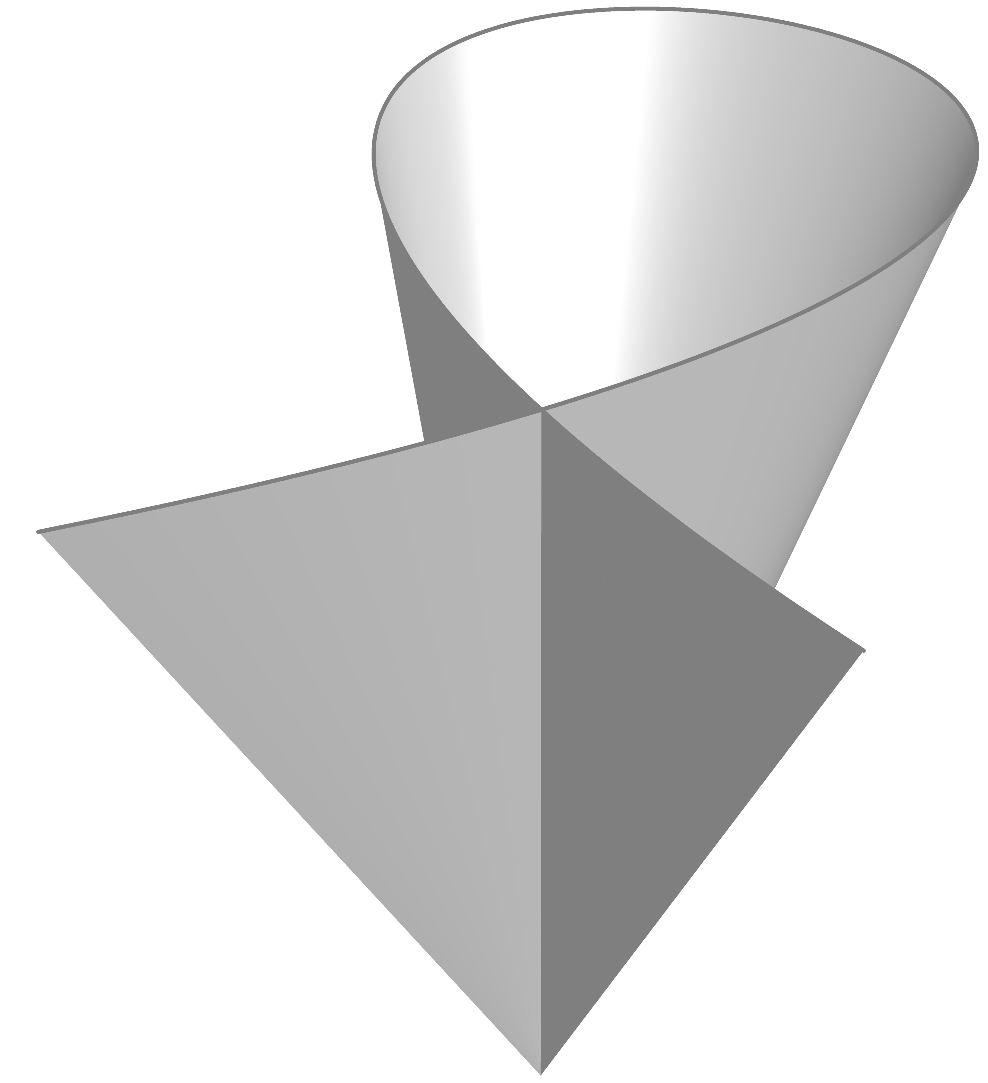
\includegraphics[width=4cm]{cone-over-cubic}
\end{center}
The recipe: given an algebraic equation in any number of variables, like \(y^2=x^2+x^3\):
\begin{enumerate}
\item 
Find the degree \(n\) of the highest term; in this example \(n=3\). 
\item
Invent a new variable, like \(z\).
\item
Multiply each term by a power of \(z\) so that the total degree of each term reaches \(n\).
\end{enumerate}
\begin{problem}{projective.plane:homogenise.2}
Homogenise \(x^2y + x^3 + y = 2x\).
\end{problem}
In sage:
\begin{sageblock}
R.<x,y,z> = PolynomialRing(QQ)
p = x^3+x*y+1
p.homogenize(z)
\end{sageblock}
yields \(\sage{p.homogenize(z)}\).

The homogenised polynomial equation \(y^2z = xz^2 + x^3\)  has all terms of degree \(3\), so if we rescale \(x,y,z\) to \(tx,ty,tz\), we rescale both sides of the equation by \(t^3\), so solutions \((x,y,z)\) rescaled remain solutions \((tx,ty,tz)\).
Thefore every solution lies on a line through the origin consisting of other solutions.
The set of solutions is a surface, which is a union of lines through the origin: a cone.
A \emph{projective plane algebraic curve}\define{projective!plane algebraic curve}\define{plane algebraic curve!projective}\define{curve!projective plane algebraic} is the set of lines through the origin satisfying a nonzero homogeneous polynomial in \(x,y,z\).
Careful: our polynomial is defined over some field \(k\), but we allow these lines through the origin to be \(\bar{k}\)-lines, i.e. have coordinates \(x,y,z\) in \(\bar{k}\) defined up to rescaling by nonzero constants in \(\bar{k}\).
\begin{example}
We can already learn from looking at the projective line instead of the projective plane.
The polynomial 
\[
p(x,y)=x^3+x^2y-2xy^2
\]
becomes 
\[
p(x,1)=x^3+x^2-2x=x(x-1)(x+2),
\]
so that 
\[
p(x,y)=x(x-y)(x+2y).
\]
So \(p(x,y)\) vanishes at precisely the points
\[
[x,y]=[0,1], [1,1], [-2,1]
\]
on the projective line.
Writing this as \(t=x/y\), these points are \(t=0,1,-2\) in \(k\cup\set{\infty}\). When \(y=1\), \(t=x/y=x\), so we might prefer to write \(p(t,1)\) here instead of \(p(x,1)\).
\end{example}
\section{Conics}
\begin{example}
Take a hyperbola \(xy=1\) in the affine plane, 
\begin{center}
\documentclass[tikz]{standalone}
\usepackage{pgfplots}\pgfplotsset{compat=1.12}
\begin{document}
\pgfplotsset{every axis/.append style={
                    axis x line=middle,    % put the x axis in the middle
                    axis y line=middle,    % put the y axis in the middle
                    axis line style={<->,color=blue}, % arrows on the axis
                    xlabel={$x$},          % default put x on x-axis
                    ylabel={$y$},          % default put y on y-axis
            }}
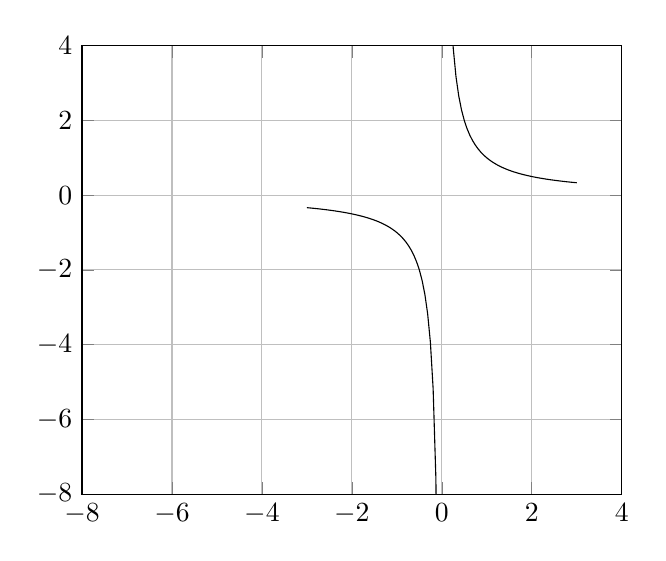
\begin{tikzpicture}
    \begin{axis}[
            xmin=-8,xmax=4,
            ymin=-8,ymax=4,
            grid=both,
            ]
            \addplot [domain=-3:-0.01,samples=50]({x},{1/x}); 
            \addplot [domain=0.01:3,samples=50]({x},{1/x}); 
    \end{axis} 
\end{tikzpicture}
\end{document}

\end{center}
and homogenise to \(xy=z^2\), as we see from three different perspectives:
\begin{center}
\includegraphicsinexample[width=8cm]{cone-over-hyperbola-p0}
\includegraphicsinexample[width=8cm]{cone-over-hyperbola-p1}
\includegraphicsinexample[width=8cm]{cone-over-hyperbola-p2}
\end{center}
If we slice the surface along a plane like \(z=2\), parallel to the plane we drew but higher up, that plane \(z=2\) intersects our surface in a dilated hyperbola.
But if we slice the surface along the plane \(x=1\), we get \(xy=z^2\) to become \(y=z^2\), a parabola:
\includegraphicsinexample[width=8cm]{cone-over-parabola}
Suitable linear changes of variable interchange the \(x\) and \(z\) axes, so suitable projective transformations identify the two affine curves: the hyperbola and the parabola.
As we will see, this ensures the two curves are birational, i.e. have isomorphic fields of rational functions.
They \emph{don't} have isomorphic rings of regular functions.

If instead we slice our surface with the plane \(x+y=1\),
\includegraphicsinexample[width=8cm]{cone-over-ellipse}
we get \(y=1-x\) plugged in to \(xy=z^2\), which simplifies to 
\[
\pr{x-\frac{1}{2}}^2 + z^2 = \frac{1}{4},
\]
a circle of radius \(\frac{1}{2}\).
So again the circle is birational to the parabola and to the hyperbola: they all have the same rational function fields.
In these pictures we can see why the conics are called \emph{conics}: they are all slices of the same cone.
\end{example}
\begin{problem}{projective.curves:rat.proj.trans}
Why is every projective transformation a birational transformation on every plane algebraic curve?
\end{problem}
\begin{answer}{projective.curves:rat.proj.trans}
Each invertible matrix
\[
A=
\begin{pmatrix}
a_{00} & a_{01} & a_{02} \\
a_{10} & a_{11} & a_{12} \\
a_{20} & a_{21} & a_{22}
\end{pmatrix}.
\]
yields a linear transformation
\begin{align*}
\begin{pmatrix}
X\\
Y\\
Z
\end{pmatrix}
&=
\begin{pmatrix}
a_{00} & a_{01} & a_{02} \\
a_{10} & a_{11} & a_{12} \\
a_{20} & a_{21} & a_{22}
\end{pmatrix}
\begin{pmatrix}
x\\
y\\
z
\end{pmatrix}\\
&=
\begin{pmatrix}
a_{00}x+a_{01}y+a_{02}z \\
a_{10}x+a_{11}y+a_{12}z \\
a_{20}x+a_{21}y+a_{22}z
\end{pmatrix}
\end{align*}
which induces the projective transformation
\begin{align*}
\begin{bmatrix}
X\\
Y\\
Z
\end{bmatrix}
&=
\begin{bmatrix}
a_{00} & a_{01} & a_{02} \\
a_{10} & a_{11} & a_{12} \\
a_{20} & a_{21} & a_{22}
\end{bmatrix}
\begin{bmatrix}
x\\
y\\
z
\end{bmatrix}
\\
&=
\begin{bmatrix}
a_{00}x+a_{01}y+a_{02}z \\
a_{10}x+a_{11}y+a_{12}z \\
a_{20}x+a_{21}y+a_{22}z
\end{bmatrix}.
\end{align*}
We can rescale. 
Scaling to get \(z=1\), and to get \(Z=1\), by dividing \(x,y,z\) by \(z\) and \(X,Y,Z\) by \(Z\), we find that in the affine planes \((z=1)\) and \((Z=1)\),
\[
\begin{pmatrix}
X\\[5pt]
Y
\end{pmatrix}
=
\begin{pmatrix}
\frac{a_{00}x+a_{01}y+a_{02}}{a_{20}x+a_{21}y+a_{22}} \\[5pt]
\frac{a_{10}x+a_{11}y+a_{12}}{a_{20}x+a_{21}y+a_{22}}
\end{pmatrix},
\]
a rational map.
The inverse is also rational, using the entries of \(A^{-1}\) in place of those of \(A\).
\end{answer}
\begin{example}
The affine curve \(x^2+y^2=-1\) has no real points on it, but has complex points.
It homogenises to \(x^2+y^2+z^2=0\), a ``sphere of zero radius'', with the origin as its only real point, but with again many complex points.
The complex linear change of variables \(X=x-iy, Y=x+iy, Z=iz\) gives us \(XY=Z^2\), the same projective curve as before.
So these curves are all birational over the complex numbers, and indeed are all identified by automorphisms of the complex projective plane.
\end{example}
\begin{problem}{projective.plane:dehomogenise}
By the same trick of homogenising and dehomogenising in various variables, draw the same sort of pictures for the circle \(x^2+y^2=1\) to see what cone it homogenises to, and what curves it makes when you intersect that cone with the planes (a) \(x=1\), (b) \(y=1\) and (c) \(z=y+1\). 
\end{problem}

\section{Points at infinity}
Take a plane algebraic curve \(C=(0=p(x,y))\) in the affine plane, i.e. the usual \(xy\)-plane.
Thinking of the projective plane as consisting of the affine plane together with some ``points at infinity'', which points at infinity lie on \(C\)?
\begin{example}
Try \(C=(y^2=x^3+x^2)\); homogeneize to \(C=(y^2z=x^3+x^2z)\).
The affine plane is \((z=1)\).
The points of the projective plane which are missing from the affine plane are those \([x,y,z]\) for which we cannot rescale \(x,y,z\) to arrange that \(z=1\), i.e. precisely those with \(z=0\).
Note that \(z=0\) hits our curve \(C\) just by plugging in \(z=0\) to the equation of \(C=(y^2z=x^3+x^2z)\), to give us \(0=x^3+0\), i.e. \(x=0\).
So to have a point at infinity \(C\), it must have \([x,y,z]=[0,y,0]\).
Since not all of \(x,y,z\) can be zero at once, we must have \(y\ne 0\) on this point, so we can rescale \(x,y,z\) by \(1/y\) to arrange \([x,y,z]=[0,1,0]\), the unique point at infinity of \(C\).

Is there an easier way?
When we put in the \(z\)-factors, we had to pop one or more into every term in \(y^2=x^3+x^2\) which was not of highest degree, i.e. all but the \(x^3\) term.
Then we set \(z=0\), killing them.
So we really just dropped all terms not of highest degree, and those highest degree terms give the equation of the points at infinity.
\end{example}
By the same reasoning:
\begin{lemma}
Take an affine curve \(C=(0=p(x,y))\), say of degree \(d\).
Expand out \(p(x,y)\) in terms of highest degree, i.e. degree exactly \(d\), and lower terms
\[
p(x,y)=p_d(x,y)+\dots
\]
The points of \(C\) which lie at infinity in the projective plane are precisely those \([x,y,z]=[x,y,0]\) with \(p_d(x,y)=0\).
\end{lemma}
\begin{problem}{projective.curves:find.the.points}
Find all points of the curve \(x^3+x^2y+xy^2+y^3+x^2=1\) which lie ``at infinity'', i.e. on the line \(z=0\) in homogeneous coordinates, over the field \(k=\C{}\).
\end{problem}
\begin{answer}{projective.curves:find.the.points}
Homogenize to \(x^3+x^2y+xy^2+y^3+x^2z=z^3\), and then set \(z=0\) to get the homogeneous equation \(x^3+x^2y+xy^2+y^3=0\).
Factor: \((x+y)(x^2+y^2)=0\).
So \(x+y=0\), i.e. \([x,-x,0]=[1,-1,0]\), or \(x^2+y^2=0\), which factors over any field \(k\) which contains an element \(i\) so that \(i^2=-1\), as \((x-iy)(x+iy)=0\), i.e. \(y=\pm ix\), so \([x,ix,0]=[1,i,0]\) and \([x,-ix,0]=[1,-i,0]\).
Hence the points of our curve that lie on the line at infinity are \([1,-1,0], [1,i,0], [1,-i,0]\).
\end{answer}
\begin{problem}{projective.curves:find.the.points.5}
Find all points of the curve \(y^2+y=x^3+x+1\) on the projective plane over the field \(k=\Z{}/5\Z{}\).
\end{problem}
\begin{answer}{projective.curves:find.the.points.5}
Start with the affine plane.
Remember (from problem~\vref{problem:polynomials:quadratic.formula}) that you can use the quadratic formula:
\[
y=\frac{-1\pm\sqrt{1-4(-x^3-x-1)}}{2}.
\]
Simplify, using \(2^{-1}=3\) and \(4=-1\), to:
\[
y=3(-1\pm\sqrt{-x^3-x})
\]
Note that \(0^2=0, 1^2=1, 2^2=4, 3^2=9=4, 4^2=16=1\), so only \(0,1,4\) have square roots.
\begin{itemize}
\item
\(x=0\): \(-x^3-x=0\), \(y=-3=2\), \([x,y,z]=[0,2,1]\).
\item
\(x=1\): \(-x^3-x=3\), no square root of \(3\), no solution.
\item
\(x=2\): \(-x^3-x=-8-2=0\), \(y=-3=2\), \([x,y,z]=[2,2,1]\).
\item
\(x=3\): \(-x^3-x=-27-3=0\), \(y=-3=2\), \([x,y,z]=[3,2,1]\).
\item
\(x=4\): \(-x^3-x=-68=2\), no square root of \(2\) no solution.
\end{itemize}
We still need the points ``at infinity''.
Homogenize: \(y^2z+yz^2=x^3+xz^2+z^3\), and set \(z=0\): \(0=x^3\), so \(x=0\), i.e. \([x,y,z]=[0,y,0]\), and rescale \(y\) to \([0,1,0]\).
Final answer: \([0,2,1], [2,2,1], [3,2,1], [0,1,0]\).
\end{answer}
\begin{problem}{projective.curves:Fermat}
Find all points of the Fermat curve at infinity.
By homogenizing, and then dehomogenizing to \((x=1)\) or to \((y=1)\), prove that the Fermat curve is smooth in the projective plane, i.e. even the points at infinity are smooth points.
\end{problem}
Restating lemma~\vref{lemma:one.variable.splits}:
\begin{lemma}\label{lemma:one.variable.splits.2}
Every nonzero homogeneous polynomial of degree \(n\) in two variables over a field \(k\) has \(n\) roots, counted with multiplicities, in \(\Proj^1_{\bar{k}}\).
\end{lemma}
Hence: 
\begin{lemma}\label{lemma:one.variable.splits.3}
Every plane algebraic curve of degree \(n\) has \(n\) points at infinity, counting multiplicities or contains the line at infinity.
\end{lemma}

\section{Breaking curves into components}
\begin{example}
The family of curves with \(y^2=ax\) contains the curve \(y^2=0\) when \(a=0\), a line.
So a family of curves of degree \(2\) contains a curve of degree \(1\).
It is natural to think of the curve being a ``double line'' when \(a=0\).
\end{example}
Similarly, we can say that a \emph{multiple component}\define{component!multiple} of a curve means a curve given by an equation which is a positive integer power of an irreducible homogeneous polynomial, say \(0=f(x,y,z)^k\) giving a component with multiplicity \(k\).
From now on, we allow plane algebraic curves to have components with positive integer multiplicities.
\begin{theorem}[Study]\define{theorem!Study}\define{Study!theorem}\label{theorem:Study}
Every algebraic curve in the projective plane has a unique decomposition into irreducible algebraic curves, its \emph{components}.
To be more precise, every nonzero homogeneous polynomial in \(3\) variables \(f(x,y,z)\) has a decomposition
\[
f=a_0 f_1^{k_1} f_2^{k_2} \dots f_n^{k_n},
\]
into a product of a nonzero constant \(a_0\) and several coprime irreducible homogeneous polynomials \(f_j(x,y,z)\) to various positive integer powers, unique up to rescaling the constant and the polynomials by nonzero constants, and writing down the polynomials in perhaps a different order.
\end{theorem}
\begin{proof}
Suppose that \(g\) is an irreducible polynomial and that \(f=0\) at every point in \(\bar{k}\) where \(g=0\). 
We want to prove that \(g\) divides \(f\).
Work in the affine plane \(z=1\).
Think of each equation as a polynomial in one variable \(x\), but with coefficients rational functions of \(y\).
By corollary~\vref{corollary:resultant.effective}, after perhaps a linear change of variables, the resultant in \(y\) vanishes just at those \(x\) values where there are simultaneous roots.
In particular, the number of different values of \(x\) where such roots occur is never more than the degree of the resultant, as a polynomial in \(x\).
For each value \(x=c\) (over \(\bar{k}\)) for which \(g(c,y)\) is not constant, the values of \(y\) at which \(g(c,y)=0\) also satisfy \(f(c,y)=0\), so the resultant vanishes.
Therefore this resultant is the zero polynomial.
If the curve where \(f=0\) is the union of distinct irreducible curves given by equations \(g_i=0\), then each of these \(g_i\) divides \(f\), so their product divides \(f\).
Apply induction on the degree of \(f\).
\end{proof}

\section{Rational morphisms}
Write any rational function
\[
\frac{b(x,y)}{c(x,y)}
\]
as a ratio of homogeneous functions by homogenizing \(b(x,y)\) and \(c(x,y)\).
But you want to make them have the same degree, so that rescaling \(x,y,z\) gives the same result, so that the function is defined on the projective plane, except where the denominator vanishes.
A \emph{rational function}\define{rational function} on the projective plane is a rational function 
\[
\frac{b(x,y,z)}{c(x,y,z)}
\]
where \(b(x,y,z)\) and \(c(x,y,z)\) are homogeneous of the same degree.
A \emph{rational function}\define{rational function} on a plane algebraic curve \((0=p(x,y,z))\) in the projective plane is a choice of rational function
\[
\frac{b(x,y,z)}{c(x,y,z)}
\]
on the projective plane, but defined only up to adding multiples of \(p(x,y,z)\) to numerator or denominator, and with \(c(x,y,z)\) not zero on some point of each component of the curve.

A \emph{rational morphism}\define{rational!morphism} \(f\colon B\to\Proj^n\) from a plane algebraic curve \(B\) is a map expressed as
\[
f(x,y,z)=
\begin{bmatrix}
X_0\\[5pt]
X_1\\[5pt]
\vdots\\[5pt]
X_n
\end{bmatrix}
=
\begin{bmatrix}
\frac{b_0(x,y,z)}{c_0(x,y,z)}\\[5pt]
\frac{b_1(x,y,z)}{c_1(x,y,z)}\\[5pt]
\vdots\\
\frac{b_n(x,y,z)}{c_n(x,y,z)}\\[5pt]
\end{bmatrix}
\]
but where we can suppose that the degree difference \(\degree{b_i}-\degree{c_i}\) is the same for each \(i=0,1,2,\dots,n\), so that when we rescale \(x,y,z\), we get the same point \(X\) of \(\Proj^n\), with these rational functions all defined at some point of each component of \(B\).
\begin{example}
The \emph{twisted cubic}\define{twisted cubic} is the rational morphism
\[
f\colon\Proj^1\to\Proj^n,
\]
given by
\[
f([x,y])=[x^3,x^2y,xy^2,y^3].
\]
\end{example}
The rational functions of a rational morphism are defined only up to scaling them all by the same rational function.
In this way, we might manage to rescale them to define a point \(f(x,y,z)\) even at points where they might at first seem to have vanishing denominators.
\begin{lemma}
Every rational morphism of a curve is defined at every regular point of that curve.
\end{lemma}
\begin{proof}
After a projective transformation, we can assume we work in the affine plane \((z=1)\).
We can rescale by denominators to arrange that all \(X_i=X_i(x,y)\) are polynomials.
But there is still the danger that all of our polynomials might vanish together at the same point \((x,y)\), so that the values \(X_i=X_i(x,y)=0\) don't define a point of projective space.
In a local parameter, on the curve, \(X_i=t^{k_i} F_i\), \(k_i\ge 0\), \(F_i\) nonzero and regular at our regular point.
Rescale by \(t^{-k}\) where \(k\) is the smallest of the \(k_i\).
\end{proof}
\begin{corollary}
A birational morphism of smooth plane algebraic curves is everywhere regular in the projective plane and a bijection between their points in the projective plane.
\end{corollary}
